\section{El juego de la vida}

En Octubre de 1970, Martin Gardner en su columna \textit{Mathematical Games} del \textit{Scientific American} \cite{Gardner1970} escribir\'ia un texto que cambiar\'ia para siempre la vida de Conway. El texto se llamar\'ia \textit{The fantastic combinations of John Conway's new solitaire game ``life''} y describir\'ia un automata celular en dos dimensiones, una suerte de juego con cero jugadores tal que, a partir de un patr\'on inicial, evolucionaba conforme a unas reglas sencillas.

La columna, adem\'as de describir el juego propon\'ia un reto, encontrar un patr\'on inicial que evolucionara de tal forma que su patr\'on creciera sin l\'imites y promet\'ia 50\$ a quien fuera el primero en encontrarla o demostrar que no existe.

La columna fue un \'exito, el juego de la vida se volvi\'o un cl\'asico de culto. Hoy en d\'ia si se busca el juego de la vida de Conway en Google la p\'agina misma empieza a jugar el juego de la vida, y si por ejemplo, se busca el juego de la vida en Youtube se puede encontrar much\'isimos ejemplos de creaciones asociadas al juego de la vida, calculadoras en el juego de la vida, relojes, otros juegos parecidos al juego de la vida, incluso hay videos como este \cite{YTEpicLife} que muestran `naves espaciales' y otros `organismos' viviendo en el juego. Como describir\'ia Siobhan Roberts en la biograf\'ia de Conway \cite{Roberts2015-ur}:

\textit{Hablando de manera pr\'actica, el juego (de la vida) empuj\'o el uso de automatas celulares y simulaciones basadas en agentes en las ciencias de la complejidad, modelando el comportamiento de todo, desde hormigas pasando por el tr\'afico, por las nubes y hasta las galaxias. Hablando de manera poco pr\'actica, el juego se convirti\'o en un cl\'asico de culto para aquellos entusiasmados en ninguna otra aplicaci\'on extravagante m\'as que perder el tiempo.\footnote{Traducci\'on del texto}}

En la biograf\'ia tambi\'en cuentan varias leyendas que se cuentan alrededor del juego de la vida. Se dice que un informe militar de Estados Unidos estim\'o que el tiempo total gastado por personas jugando el juego de la vida en el trabajo equival\'ia a millones de dolares perdidos, tambi\'en se dice que en el momento en que el juego fue m\'as viral, en $\frac{1}{4}$ de los computadores del mundo se jugaba el juego de la vida.

Fue tanta la fama del juego de la vida que su creador, Jhon Horton Conway, lleg\'o a decir que odiaba el juego de la vida ya que cada vez que se mencionaba su nombre en algun art\'iculo matem\'atico lo \'unico que se mencionaba era el juego de la vida, casi que eclipsando todos los otros logros matem\'aticos que \'el hab\'ia hecho \cite{YTNumberphileConway}.

\subsection{Los inicios}

La biograf\'ia de Conway \cite{Roberts2015-ur} cuenta que la idea del juego de la vida comenz\'o desde mucho antes. Seg\'un Stephen Wolfram \cite{MathematicalArtist2022}, Conway le cont\'o que en ese tiempo hab\'ia sido contratado como profesor de l\'ogica pero que ese no era su campo de investigaci\'on principal. Conway se interes\'o entonces en los aut\'omatas, su plan era encontrar una buena enumeraci\'on de las funciones recursivas. En ese entonces Conway ten\'ia una copia del libro \textit{Automata Studies} \cite{Shannon1956}, una recolecci\'on de ensayos sobre aut\'omatas recopilados por Claude Shannon y Jhon McCarthy, los padres de la teor\'ia de la informaci\'on y de la inteligencia artificial respectivamente. Conway cuenta que fueron las ideas de c\'omo los aut\'omatas podr\'ian en alg\'un momento simular cosas complejas como el cerebro humano, o incluso, podr\'ian replicarse a s\'i mismas. John von Neumann por ejemplo, ve\'ia un potencial en los aut\'omatas inmenso, pensaba en que en alg\'un momento se podr\'ia crear una m\'aquina que pudiera crear otras m\'aquinas y utilizarlas colonizando otros planetas. La idea que Von Neumann desarrollaba, ya m\'as abstra\'ida al terreno matem\'atico, era sobre un aut\'omata celular dos dimensional con la posibilidad de replicarse a s\'i mismo, la idea fue publicada despu\'es de su muerte en su libro \textit{Theory of self-reproducing automata} \cite{Von_Neumann1967-ma}. Sin embargo Conway le ve\'ia un problema al resultado de Von Neumann, cada celda del aut\'omata podr\'ia estar en un total de 29 estados, lo que \'el consideraba muy complejo. Como dir\'ia el en su biograf\'ia:

\textit{Parec\'ia terriblemente complicado. Lo que me emociona son las cosas que tienen una maravillosa simplicidad.}

Y as\'i empez\'o una busqueda hac\'ia un automata, universal (que pueda replicar cualquier m\'aquina), y adem\'as que fuera lo m\'as simple posible. Algo que describir\'ia como su \textit{Jugendtraum}, su sueño de juventud.

\subsection{FRACTRAN}

Su primera aproximaci\'on fue la creaci\'on del lenguaje de programaci\'on \textbf{FRACTRAN}, una idea 1-dimensional de hacer una m\'aquina universoal. El nombre surge de una combinaci\'on del nombre del lenguaje de programaci\'on \textbf{FORTRAN} (IBM's Mathematical \textbf{For}mula \textbf{Tran}slating System), con la palabra fracci\'on, que es b\'asicamente como se codifican los programas en este lenguaje.

Los programas en FRACTRAN se escriben como una lista finita de fracciones enteras, por ejemplo, 
\[
    \left(\frac{1}{2}, \frac{1}{3}, \frac{1}{5}\right).
\]
El programa siempre recibe solamente un n\'umero entero $n$ y procede de tal forma que
\begin{enumerate}
    \item Encuentra la primera fracci\'on $f$ de izquierda a derecha tal que $nf$ sea un n\'umero entero.
    \item Reemplaza el n\'umero $n$, por el n\'umero $nf$.
    \item Repite el procedimiento desde el punto $(1)$ hasta que no exista tal fracci\'on.
\end{enumerate}

Por ejemplo, supongamos que nuestro programa es el que se escribi\'o antes y nuestro n\'umero es $n_1= 10$. La primera fracci\'on de izquierda a derecha tal que multiplicada por $n_1$ es entero es la fracci\'on $f = \frac{1}{2}$, por lo tanto reemplazamos nuestro $n_1$ por $n_2 = n_1/2 = 5$, y repetimos. F\'ijese que ahora que $n_2 = 5$, ni la primera fracci\'on ni la segunda multiplicadas por $n$ dan un n\'umero entero, en cambio la tercera, $f=\frac{1}{5}$, s\'i da un n\'umero entero, por lo tanto reemplazamos $n_2$ por $n_3 = n_2/5= 1$. Ahora, con nuestro \'ultimo $n_3 = 1$, tenemos que ninguna de las fracciones multiplicadas por $n_3 = 1$ nos dan un n\'umero entero, por lo tanto nuestro programa ha finalizado y ha dado como resultado $1$. En general, se puede representar el programa con la tabla

\begin{center}
    \begin{tabular}{|c|M{3cm}|M{3cm}|M{3cm}|}
        \hline
        \# & N & f \\
        \hline\hline
        1 & 10 & \frac{1}{2} \\
        \hline
        2 & 5 & \frac{1}{5} \\
        \hline
        3 & 1 & \text{\textbf{FINAL}} \\
        \hline
    \end{tabular}
\end{center}

Si bien el FRACTRAN parece simple, tiene la capacidad de hacer cualquier procedimiento que un computador cualquiera puede hacer, en palabras de la teor\'ia de la computaci\'on, FRACTRAN es Turing completo. 

Mostremos por ejemplo que se pueden sumar n\'umeros. Considere el programa que consiste en la fracci\'on
\[
    \left(\frac{2}{3}\right).
\]

Ahora por ejemplo corramos el programa con el n\'umero $n_1 = 72 = 2^33^2$. Entonces nuestro programa correr\'ia de manera que

\begin{center}
    \begin{tabular}{|c|M{3cm}|M{3cm}|M{3cm}|}
        \hline
        \# & N & \text{Descomposici\'on} & f \\
        \hline\hline
        1 & 72 & 2^33^2 & \frac{2}{3} \\
        \hline
        2 & 48 & 2^43^1 & \frac{2}{3} \\
        \hline
        2 & 32 & 2^5 & \text{\textbf{FINAL}} \\
        \hline
    \end{tabular}
\end{center}

En este caso, si nos fijamos en la descomposici\'on, podemos ver que en cada paso del algoritmo lo que est\'a pasando es que el exponente que acompaña el factor $3$ se va reduciendo en $1$ mientras el que acompaña el factor de $2$ se va aumentando en $1$, y esto se repite hasta que no haya exponente del factor de $3$. En otras palabras, si $n_1 = 2^a3^b$, entonces en el siguiente paso lo que pasar\'a es que $n_2 = 2^{a+1}3^{b-1}$, y lo seguir\'a haciendo hasta que $n_k = 2^{a+b}3^{b-b} = 2^a+b$. Lo que est\'a sucediendo es que a este programa ingresan n\'umeros de la forma $2^a3^b$ y salen n\'umeros de la forma $2^{a+b}$, es decir, se est\'an sumando los n\'umeros $a$ y $b$.

En general, el lenguaje de FRACTRAN se basa en que los valores se guardaran en los exponentes de los n\'umeros primos. Por ejemplo en este programa, si queremos saber la suma de dos n\'umeros $a$ y $b$ entonces lo que tendremos que hacer es poner en el programa el n\'umero $2^a3^b$ y la respuesta la obtendremos en el exponente del n\'umero $2$ del resultado que nos dar\'a el programa, en este caso el n\'umero $2^{a+b}$. En este sentido las `variables' en FRACTRAN son n\'umeros primos y sus `valores' son los exponentes que los acompañan, cada fracci\'on es entonces una instrucci\'on para quitar un valor fijo a algunas variables y agregarle un valor fijo a otras variables.

Teniendo esto en cuenta podemos diseñar diferentes algoritmos para mostrar su poder computacional. As\'i como se puede sumar tambi\'en se puede restar, analizemos el programa

\[
    \left(\frac{1}{6}\right).
\]

Aqu\'i tenemos que si corremos el programa con el n\'umero $2^a3^b$, el resultado depende de cu\'al n\'umero es menor. Si $a > b$, entonces el programa nos dar\'a como resultado $2^{a-b}$, si  $a < b$, entonces el programa nos dar\'a como resultado $3^{b-a}$, y si $a = b$, entonces lo que pasar\'ia es que el resultado ser\'ia $1$. Aqu\'i en este programa no solamente tenemos una forma de restar n\'umeros, sino tambi\'en una forma de compararlos.

Tambi\'en podemos pensar en c\'omo se diseñar\'ia una condici\'on en FORTRAN, una estructura IF. Supongamos que el programa tiene como entrada un n\'umero $2^a3^b5^c$ y queremos diseñarlo tal que si $c = 1$ entonces el programa suma $a+b$, y si $c = 0$ el programa los resta. Considere entonces el programa

\[
    \left(\frac{2\times 7}{3\times 5},\frac{5}{7},\frac{1}{2\times 3}\right) = \left(\frac{14}{15},\frac{5}{7},\frac{1}{6}\right).
\]

Aqu\'i añadimos dos `variables' m\'as, los n\'umeros primos $5$ y $7$. La funci\'on de estos dos es intercalarse para que cada vez que haya valor en el $5$ se sumen, y se utiliza el $7$ para de cierto modo guardar el valor del $5$ puesto que cada vez que se suman el $5$ va disminuyendo su valor en $1$. Si el $5$ no est\'a en la entrada, es decir, si $c = 0$, entonces se puede ver que el programa va directo a la fracci\'on $\frac{1}{2\times 3} = \frac{1}{6}$, es decir, la fracci\'on de restar. Veamos entonces un ejemplo, veamos los pasos del programa con el n\'umero $2^33^25^1$.

\begin{center}
    \begin{tabular}{|c|M{3cm}|M{3cm}|M{3cm}|}
        \hline
        \# & N & \text{Descomposici\'on} & f \\
        \hline\hline
        1 & 360 & 2^33^25^1 & \frac{2\times 7}{3\times 5} \\
        \hline
        2 & 336 & 2^43^17^1 & \frac{5}{7} \\
        \hline
        2 & 240 & 2^43^15^1 & \frac{2\times 7}{3\times 5}\\
        \hline
        2 & 224 & 2^57^1 & \frac{5}{7} \\
        \hline
        2 & 160 & 2^55^1 & \text{\textbf{FINAL}} \\
        \hline
    \end{tabular}
\end{center}

Un diseño interesante es ver c\'omo se puede utilizar todo esto para multiplicar dos n\'umeros. Ya teniendo un programa que sume dos n\'umeros, si queremos un programa que multiplique necesitaremos entonces que el programa sume dos n\'umeros varias veces. Veamos como podr\'iamos diseñarlo, supongamos que de entrada del programa tenemos un n\'umero $2^a3^b$, y que queremos como resultado $5^{ab}$. Una forma de intentarlo ser\'ia, cada vez que le quitemos uno al exponente de $2$ vamos a agregar $b$ al exponente de $5$, para esto podemos utilizar las condicionales que desarrollamos en el ejemplo anterior: cada vez que le quitemos uno al exponente de $2$ vamos a agregarle $1$ al exponente de $11$ que nos indicar\'a que tenemos que sumarle $b$ al exponente de $5$. Por ahora nuestro programa se ver\'ia as\'i

\[
    \left(\dots,\frac{1}{11},\frac{11}{2},\dots\right).
\]

La fracci\'on $\frac{1}{11}$ la agregamos para limpiar el $11$ cuando terminemos de sumarle $b$ al exponente de $5$.

Ahora, si queremos sumar $b$ al exponente de $5$ podemos hacerlo de un modo parecido a la condici\'on anterior. En este caso tendr\'iamos 

\[
    \left(\frac{5\times 13}{3\times 11}, \frac{11}{13}, \frac{1}{11},\frac{11}{2}\right).
\]
Este algoritmo tiene un problema, si bien le añadimos $b$ a $5$, solo lo hacemos una vez, ya que despues de la primera vez el exponente de $3$ queda en $0$. Lo que podemos hacer para arreglar esto, es añadir una `variable' m\'as que nos ayude a guardar el valor de $3$ en cada iteraci\'on, lo podemos hacer con el n\'umero $7$. Algo as\'i nos quedar\'ia

\[
    \left(\frac{5\times 13\times 7}{3\times 11}, \frac{11}{13}, \frac{1}{11}, \frac{3}{7},\frac{11}{2}\right),
\]

este programa de FRACTRAN nos devuelve como resultado $5^ab3^b$, por lo tanto, si queremos limpiar el exponente de $3$ lo que podr\'iamos hacer es poner la fracci\'on $1/3$ al final, as\'i, nuestro programa final queda

\[
    \left(\frac{5\times 13\times 7}{3\times 11}, \frac{11}{13}, \frac{1}{11}, \frac{3}{7},\frac{11}{2}, \frac{1}{3}\right) = \left(\frac{455}{33}, \frac{11}{13}, \frac{1}{11}, \frac{3}{7},\frac{11}{2}, \frac{1}{3}\right),
\]

y nos queda id\'entico al programa definido en la p\'agina de Wikipedia de FRACTRAN \cite{wiki:FRACTRAN}.

Lo sorprendente de FRACTRAN es que su simplicidad permita generar cualquier programa posible, uno de los ejemplos que Conway da en su art\'iculo \cite{Conway1987} en el que da a conocer FRACTRAN es el de un programa de $14$ fracciones que genera los n\'umeros primos sucesivamente 
\[
    {\displaystyle \left({\frac {17}{91}},{\frac {78}{85}},{\frac {19}{51}},{\frac {23}{38}},{\frac {29}{33}},{\frac {77}{29}},{\frac {95}{23}},{\frac {77}{19}},{\frac {1}{17}},{\frac {11}{13}},{\frac {13}{11}},{\frac {15}{14}},{\frac {15}{2}},{\frac {55}{1}}\right)}.
\]

Sin embargo, esto no era suficiente para lograr su \textit{Jugendtraum}, Conway estaba buscando algo con un poco m\'as de vida, algo \'organico. El lo describir\'ia como un sistema sin ning\'un plan de desarrollo, un sistema no planeado.

\subsection{Life}

El juego de la vida pas\'o por much\'isimas versiones, mientras FRACTRAN era una idea de hacer un aut\'omata en cierto sentido 1-dimensional, Conway desech\'o la idea y se concentr\'o en hacer aut\'omatas 2-dimensionales.

Empezaron a pensar en t\'erminos de vida y muerte, la idea era tener reglas para que una celda `viviera' y para que una celda `muriera', en ese sentido la celda ten\'ia dos estados. La idea era encontrar un buen balance entre las dos reglas, si las reglas sobre la muerte eran muy estrictas entonces todas las celdas terminar\'ian muertas pasados unas cuantas iteraciones, y si las reglas de la vida eran muy suaves entonces los patrones crecer\'ian much\'isimo sin dar tiempo a poder hacer algo \'util con ellos.

En la pen\'ultima versi\'on del juego de la vida, las celdas ten\'ian tres posibles estados, la idea era darles un `sexo' a las celdas vivas, dando los posibles estado `macho', `hembra' y `muerto'. En el blog de Tanya Khonakova \cite{blog:tanyakhovanova}, Conway cuenta que los nombres que les pusieron eran `obispos' y `actrices' seg\'un un chiste brit\'anico. El problema que ten\'ia esta idea era que para que las reglas estuvieran bien balanceadas, las celdas que nacieran necesitaban que hubiera tres celdas vivos adyacentes, en este caso tendr\'ia que haber dos `padres' con el mismo sexo y la nueva celda tendr\'ia que tener el sexo contrario para que hubiera un balance entre ambos sexos, era un tanto complicado y al final vieron que el sexo no ten\'ia m\'as efecto que determinar el sexo de la nueva celda, por lo tanto la solucion que encontraron fue hacer un aut\'omata asexual, solamente dos estados, `vivos' y `muertos'.

El juego de la vida se juega en un tablero dos dimensional conformado por celdas, como un tablero de Go pero infinito. El juego empieza con un estado inicial y va evolucionando conforme a las reglas. Cada celda tiene 8 celdas adyacentes, cuatro que comparten un lado y cuatro que comparten solamente un v\'ertice, es decir, dos horizontales, dos verticales, y cuatro en diagonal. Las reglas del juego son:

\begin{enumerate}
    \item \textbf{Regla de nacimiento:} Si una celda est\'a muerta en el tiempo $t$, y la celda tiene exactamente $3$ celdas vecinas que est\'an vivas, entonces la celda se convierte en una celda viva en el tiempo $t+1$.
    \item \textbf{Regla de muerte:} Si una celda viva en el tiempo $t$ tiene menos que $2$ vecinos vivos, la celda muere por soledad en el tiempo $t+1$. Si una celda viva en el tiempo $t$ tiene m\'as que $3$ vecinos vivos, la celda muere por hacinamiento en el tiempo $t+1$.
    \item \textbf{Regla de supervivencia:} Si una celda viva tiene exactamente $2$ o $3$ celdas vivas vecinas, entonces la celda sigue viva en el tiempo $t+1$.
\end{enumerate}

Hagamos un ejemplo. Supongamos que de estado inicial tenemos tres celdas vivas puestas verticalmente, como en la figura \ref{figure:blinker}. Despu\'es del primer paso, la celda que est\'a en el medio ten\'ia dos celdas adyacentes vivas, entonces la celda sobrevivira, mientras que las celdas de arriba y abajo solo ten\'ian una celda vecina viva, por lo tanto estas celdas morir\'an en la siguiente iteraci\'on. Sin embargo, las celdas que se encuentran justo a los lados derecho e izquierdo de la celda del frente ten\'ian exactamente tres vecinos vivos, por lo tanto nacer\'an en el siguiente paso.

\begin{figure}[h]
    \centering
    \begin{subfigure}{0.4\textwidth}
        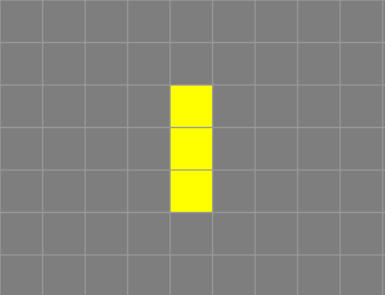
\includegraphics[width=\textwidth]{images/life-1.png}
    \end{subfigure}
    \begin{subfigure}{0.4\textwidth}
        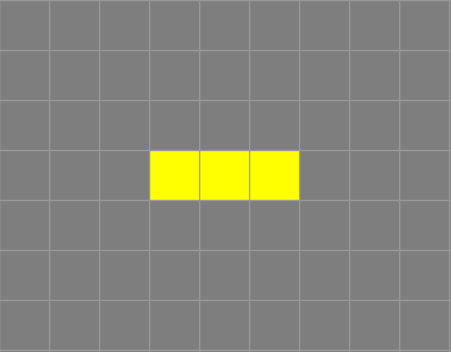
\includegraphics[width=\textwidth]{images/life-2.png}
    \end{subfigure}
    \caption{En la izquierda se muestra la configuraci\'on en el paso $t=0$, a la derecha en la iteraci\'on siguiente $t=1$. A esta figura se le conoce como \textit{blinker}.}
    \label{figure:blinker}
\end{figure}


Los \textit{blinker} de la figura \ref{figure:blinker} tienen la propiedad de que se repiten, es decir, vuelven a su estado inicial. En el caso del \textit{blinker} se puede ver que por simetr\'ia, pasa de ser tres celdas verticales a ser tres celdas horizontales y viceversa. A los patrones que tienen la propiedad de volver a su estado inicial se les llama \textit{osciladores}, y a la cantidad de pasos que se demoran para volver a su estado inicial se le llama \textit{periodo}.

\begin{figure}[h]
    \centering
    \begin{subfigure}{0.3\textwidth}
        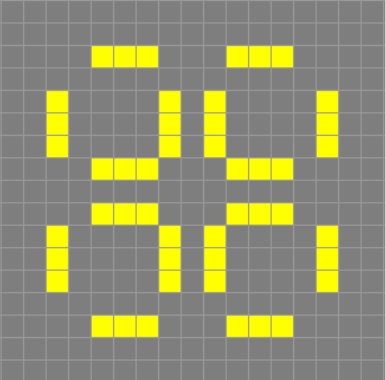
\includegraphics[width=\textwidth]{images/life-pulsar-1.png}
    \end{subfigure}
    \begin{subfigure}{0.3\textwidth}
        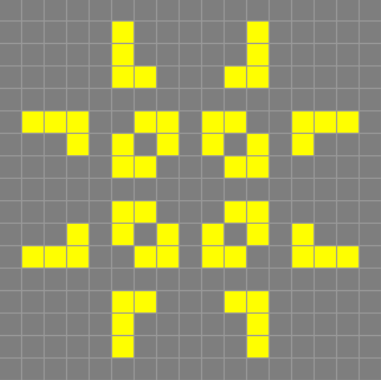
\includegraphics[width=\textwidth]{images/life-pulsar-2.png}
    \end{subfigure}
    \begin{subfigure}{0.3\textwidth}
        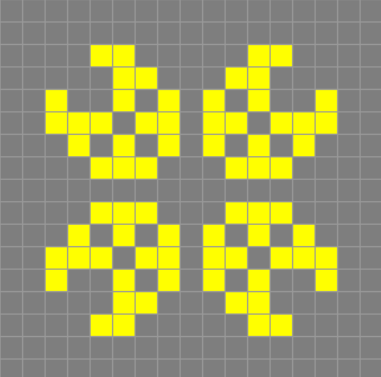
\includegraphics[width=\textwidth]{images/life-pulsar-3.png}
    \end{subfigure}
    \caption{En la figura se pueden ver los pasos de la evoluci\'on de un patr\'on llamado \textit{pulsar}. Es un oscilador de periodo 3, por lo tanto despu\'es del tercer paso vuelve a su estado inicial.}
    \label{figure:pulsar}
\end{figure}

Adem\'as de los osciladores, tambi\'en exist\'ian otros patrones que no cambiaban en absoluto al pasar el tiempo, a estos patrones se les llama \textit{estacionarios}. El m\'as simple de estos patrones es el \textit{bloque}, conformado por cuatro celdas vivas unidas en forma de cuadrado, ninguna muere porque cada una est\'a en contacto con exactamente $3$ celdas vivas mientras que las celdas muertas alrededor solamente est\'an en contacto con $2$ celdas vivas, por lo tanto no pueden nacer. Se puede ver el bloque de primeras en la figura \ref{figure:stationary}.

\begin{figure}[b]
    \centering
    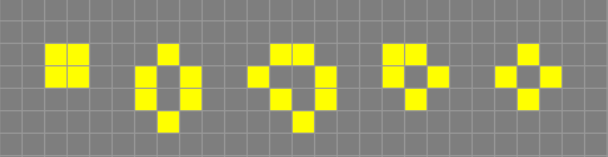
\includegraphics[width=0.7\textwidth]{images/life-stationary.png}
    \caption{Cinco patrones estacionarios, es decir, ninguno cambia con el tiempo. Sus nombres izquierda a derecha: un \textit{bloque}, una \textit{colmena}, una \textit{tajada de pan}, un \textit{bote}, un \textit{balde}.}
    \label{figure:stationary}
\end{figure}

De las primeros patrones que se estudiaron, problablemente los m\'as interesantes son los llamados \textit{Matusal\'en}, en referencia al personaje m\'as longevo de la biblia. Estos patrones tienen en com\'un que evolucionan por largos periodos de tiempo antes de estabilizarse, es decir, en volverse figuras conocidas, como los osciladores o las figuras estacionarias. El primer Matusal\'en que se encontr\'o fue el R-pentomin\'o (ver figura \ref{figure:pentomino-r}), que tambi\'en fue una de las primeras evidencias de la complejidad que podr\'ia traer el juego de la vida. El R-pentomin\'o se demora 1103 iteraciones en estabilizarse, por lo tanto, fue un gran desaf\'io para los primeros investigadores del juego de la vida, que b\'asicamente hac\'ian toda su investigaci\'on en tableros de Go y a mano.

\begin{figure}[h]
    \centering
    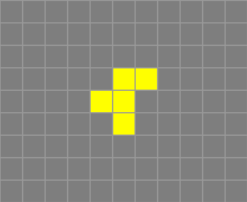
\includegraphics[width=.4\textwidth]{images/life-r-pentomino.png}
    \caption{El R-pentomin\'o.}
    \label{figure:pentomino-r}
\end{figure}

La complejidad del R-pentomin\'o se descubri\'o porque Conway y su equipo estaban probando patrones simples, empezaron con los pentomin\'os y se dieron cuenta que la mayor\'ia de ellos se estabilizaba apenas pasaban unas cuantas iteraciones, todos los dem\'as pentomin\'os con menos de 6 celdas vivas se estabilizan antes de la onceava iteraci\'on. Como Conway y su equipo hac\'ia el trabajo de revisar los patrones de manera an\'aloga, se realizaban muchos errores. Al equipo de ellos lleg\'o a ayudarlos Richard Guy, un matem\'atico de Cambridge, que tuvo el trabajo de revisar y escrutinar la evoluci\'on de los patrones de los que a\'un no conoc\'ian todo, entre esos, el R-pentomin\'o. En la iteraci\'on n\'umero $69$, Richard Guy atisb\'o un nuevo patr\'on que se separaba del caos formado por el R-pentomin\'o y en las siguientes generaciones se apartaba m\'as y m\'as, cada vez como si caminara a trav\'es del tablero. Guy se lo mostr\'o a Conway, y este \'ultimo lo bautiz\'o \textit{glider}\footnote{Su traducci\'on al espan\~ol ser\'ia planeador, haciendo referencia a los aviones planeadores}.

\begin{figure}[b]
    \centering
    \begin{subfigure}{0.15\textwidth}
        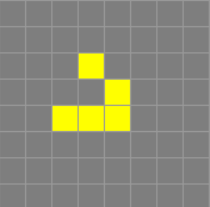
\includegraphics[width=\textwidth]{images/life-glider-1.png}
    \end{subfigure}
    \begin{subfigure}{0.15\textwidth}
        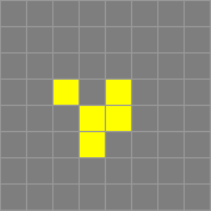
\includegraphics[width=\textwidth]{images/life-glider-2.png}
    \end{subfigure}
    \begin{subfigure}{0.15\textwidth}
        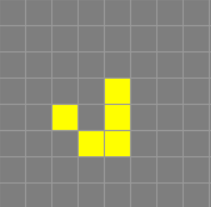
\includegraphics[width=\textwidth]{images/life-glider-3.png}
    \end{subfigure}
    \begin{subfigure}{0.15\textwidth}
        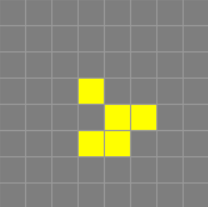
\includegraphics[width=\textwidth]{images/life-glider-4.png}
    \end{subfigure}
    \begin{subfigure}{0.15\textwidth}
        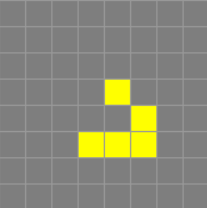
\includegraphics[width=\textwidth]{images/life-glider-5.png}
    \end{subfigure}
    \caption{La evoluci\'on del \textit{glider}. Despu\'es de 4 iteraciones se transforma por una copia del mismo pero una casilla corrida a la derecha y abajo.}
\end{figure}

Este \textit{glider} cambiar\'ia el curso que tomar\'ia el juego de la vida. Para que un aut\'omata se asemeje a un computador tiene que poder enviar informaci\'on de alguna manera, cuando Conway y su equipo encontr\'o el \textit{glider} se imaginaron que podr\'ian enviar informaci\'on mediante ellos. Para poder hacerlo, igual que se hace con el voltaje en la vida real, se necesita una forma de generar los \textit{gliders} en masa y controladamente, algo as\'i como un ca\~non de gliders. En el art\'iculo de Gardner \cite{Gardner1970}, el reto era para cualquier patr\'on que creciera sin l\'imites, pero hac\'ia referencia a que una pistola de gliders ser\'ia lo mejor para la investigaci\'on, pues una pistola de gliders tambi\'en ser\'ia un patr\'on que crecer\'ia sin l\'imite.

En Noviembre del a\~no en que sali\'o la columna de Gardner (1970), un equipo del MIT liderado por Bill Gosper, un matem\'atico y programador estadounidense, se gan\'o el premio propuesto en la columna al descubrir/inventar una pistola de gliders ahora conocida como la \textit{Gosper Glider gun} (ver figura \ref{figure:gosper-gun}). 

\begin{figure}[h]
    \centering
    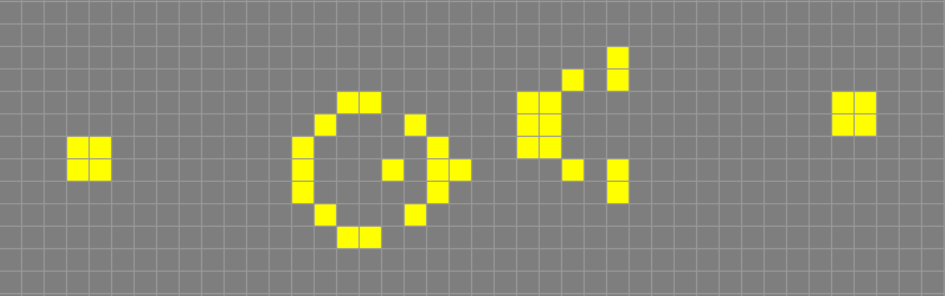
\includegraphics[width=.8\textwidth]{images/life-gosper-gun.png}
    \caption{La \textit{Gosper glider gun}. Genera un glider en la iteraci\'on 15, y a partir de esa genera un glider cada 30 iteraciones.}
    \label{figure:gosper-gun}
\end{figure}

Despu\'es de la carrera por encontrar una pistola de gliders, vino la carrera para mostrar que el juego de la vida era universal, es decir, que se pod\'ia generar un computador en el juego de la vida. Despu\'es del glider se econtraron muchas otras `naves espaciales', muchas m\'as grandes, y se estudi\'o tambi\'en c\'omo sus interacciones (o choques) podr\'ian ser \'utiles para mostrar la universalidad.

Una forma de, por ejemplo, hacer una compuerta l\'ogica NOT es utilizando estas propiedades. Si dos gliders se chocan de una manera precisa, resultara en la destrucci\'on de los dos gliders, tal como se muestra en la figura \ref{figure:glider-collission}. Por lo tanto, si tenemos una corriente de gliders a la cual le queremos sacar el NOT, lo que podemos hacer es chocarla con una corriente de gliders constante, de modo que si no se chocan la corriente constante seguir\'a produciendo y si en cambio s\'i se chocan, todos los producidos por la corriente se destruir\'an.

\begin{figure}[b]
    \centering
    \begin{subfigure}{0.22\textwidth}
        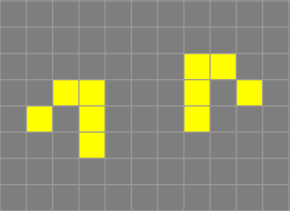
\includegraphics[width=\textwidth]{images/life-glider-collission-1.png}
    \end{subfigure}
    \begin{subfigure}{0.22\textwidth}
        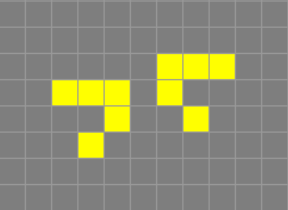
\includegraphics[width=\textwidth]{images/life-glider-collission-2.png}
    \end{subfigure}
    \begin{subfigure}{0.22\textwidth}
        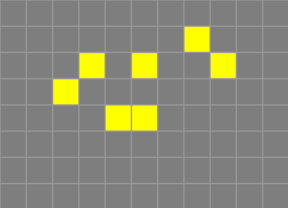
\includegraphics[width=\textwidth]{images/life-glider-collission-3.png}
    \end{subfigure}
    \begin{subfigure}{0.22\textwidth}
        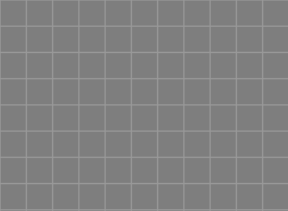
\includegraphics[width=\textwidth]{images/life-glider-collission-4.png}
    \end{subfigure}
    \caption{Dos gliders llendo en direcciones opuestas que chocan destruyendose mutuamente. Fotos tomadas al tiempo t=0,2,4,6, respectivamente de izquierda a derecha.}
    \label{figure:glider-collission}
\end{figure}

Si bien la existencia de compuertas l\'ogicas de por s\'i no implica que el juego de la vida fuera universal, se fueron descubriendo varios patrones que implicaban de cierta manera que se pod\'ia construir un computador en el juego de la vida. Esto es, se descubrieron varios patrones para poder guardar informaci\'on, igualmente todo basado en gliders.

Un mes despu\'es de que Bill Gosper descubriera la pistola de gliders que lleva su nombre, Conway le escribi\'o una carta a Martin Gardner que dec\'ia \cite{Roberts2015-ur}:
\newpage

\textit{Querido MG,} 

\textit { Espero que esta carta no te llegue muy tarde - el correo parece que se demora mucho en llegarte. Retras\'e esta carta hasta ahora porque quer\'ia completar mi prueba de que EL JUEGO DE LA VIDA ES UNIVERSAL.}

Si bien Conway nunca public\'o su prueba de que el juego de la vida es universal, el juego se volvi\'o tan famoso que hasta la fecha se han hecho un mont\'on de construcciones en el juego de la vida que lo prueban. En ese entonces se estimaba que para hacer un computador en el juego de la vida se necesitar\'ia millones de celdas, sin embargo, ahora se sabe, gracias a descubrimientos hechos por comunidades en l\'inea, que no se necesita tantas celdas para hacer un computador.